\documentclass[aspectratio=169]{beamer}

\usepackage{amsmath}
\usepackage{amssymb}
\usepackage{graphicx}
\usepackage{tikz}
\usetikzlibrary{shapes.geometric, arrows.meta, positioning}

\definecolor{coolpurple}{HTML}{7f65a0}
\definecolor{lightpurple}{HTML}{ede8f5}
\definecolor{darktext}{HTML}{1a1a2e}
\definecolor{highlightpurple}{HTML}{5a3e82}

\setbeamercolor{normal text}{fg=darktext, bg=white}
\setbeamercolor{structure}{fg=coolpurple}
\setbeamercolor{frametitle}{fg=white, bg=coolpurple}
\setbeamercolor{title}{fg=white, bg=coolpurple}
\setbeamercolor{subtitle}{fg=white}
\setbeamercolor{date}{fg=coolpurple}
\setbeamercolor{author}{fg=coolpurple}
\setbeamercolor{item}{fg=coolpurple}
\setbeamercolor{subitem}{fg=coolpurple!70!black}
\setbeamercolor{block title}{bg=coolpurple, fg=white}
\setbeamercolor{block body}{bg=lightpurple, fg=darktext}
\setbeamercolor{alerted text}{fg=highlightpurple}

\setbeamertemplate{itemize item}{\color{coolpurple}$\blacktriangleright$}
\setbeamertemplate{itemize subitem}{\color{coolpurple!70}$\bullet$}
\setbeamertemplate{navigation symbols}{}

\setbeamertemplate{footline}[frame number]

\newcommand{\hl}[1]{\textcolor{coolpurple}{\textbf{#1}}}

\title{Multi-Modal Social Behaviour Analysis}
\subtitle{M1 Presentation - March 29, 2026}
\author{Lado Turmanidze, Luka Javakhishvili, Mariami Gadelia, Keso Chikhladze}
\institute{\small{Supervisors: Dr. Philipp Müller \& Beso Mikaberidze}}
\date{March 29, 2026}

\begin{document}
	
	\begin{frame}
		\titlepage
	\end{frame}
	
	\begin{frame}{Today's Agenda}
		\begin{enumerate}
			\item \textbf{What we are doing} - project goal and datasets
			\item \textbf{The core architecture} - BiMamba-TTA
			\item \textbf{Current work} - adapting TTA to regression and modality analysis
		\end{enumerate}
	\end{frame}
	
	\begin{frame}{\textsc{Part 1:} What We Are Doing}
		\begin{center}
			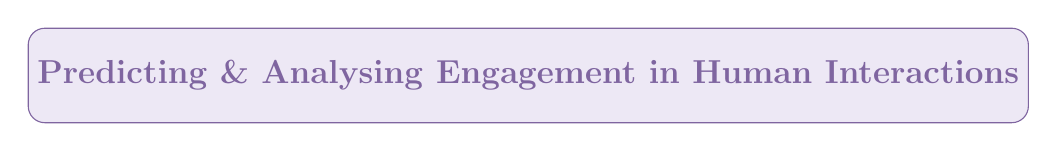
\begin{tikzpicture}
				\node[draw=coolpurple, fill=lightpurple, rounded corners=6pt,
				minimum width=10cm, minimum height=1.2cm,
				font=\large\bfseries, text=coolpurple] {
					Predicting \& Analysing \textbf{Engagement} in Human Interactions
				};
			\end{tikzpicture}
		\end{center}
		\begin{columns}[onlytextwidth]
			\begin{column}{0.60\textwidth}
				\begin{itemize}
					\item We work on \hl{engagement prediction} and \hl{behavioural personalisation} in expert-novice dyadic interactions.
					\item Multi-modal inputs: video, audio, text, body pose, facial landmarks - all fused together.
					\item \textbf{Our task:} predict a continuous engagement score $y \in [0,1]$ frame-wise at \textbf{25 Hz}.
					\item Key challenge: \hl{cross-cultural generalisation} between European (NoXi) and East-Asian (NoXi+J) sessions.
				\end{itemize}
			\end{column}
			\begin{column}{0.38\textwidth}
				\raggedright
				\scalebox{0.65}{
					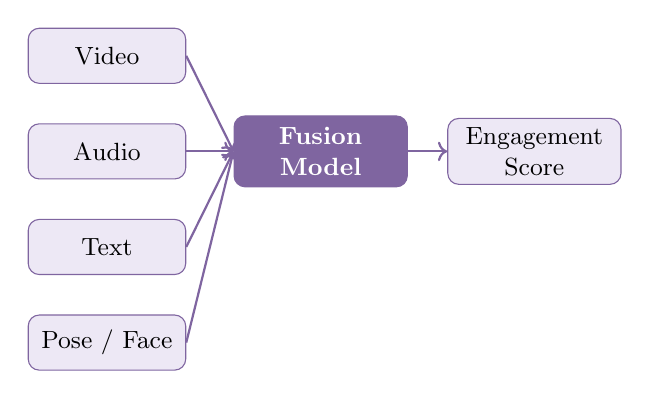
\begin{tikzpicture}[node distance=0.5cm, font=\small]
						\node[draw=coolpurple, fill=lightpurple, rounded corners, minimum width=2cm, minimum height=0.7cm, align=center] (video) {Video};
						\node[draw=coolpurple, fill=lightpurple, rounded corners, minimum width=2cm, minimum height=0.7cm, align=center, below=of video] (audio) {Audio};
						\node[draw=coolpurple, fill=lightpurple, rounded corners, minimum width=2cm, minimum height=0.7cm, align=center, below=of audio] (text) {Text};
						\node[draw=coolpurple, fill=lightpurple, rounded corners, minimum width=2cm, minimum height=0.7cm, align=center, below=of text] (pose) {Pose / Face};
						\node[draw=coolpurple, fill=coolpurple, rounded corners, minimum width=2.2cm, minimum height=0.9cm, align=center, right=0.6cm of audio, text=white, font=\small\bfseries] (model) {Fusion\\Model};
						\node[draw=coolpurple, fill=lightpurple, rounded corners, minimum width=2.2cm, minimum height=0.7cm, align=center, right=0.5cm of model] (out) {Engagement\\Score};
						\foreach \n in {video, audio, text, pose}
						\draw[->, thick, coolpurple] (\n.east) -- (model.west);
						\draw[->, thick, coolpurple] (model) -- (out);
					\end{tikzpicture}
				}
			\end{column}
		\end{columns}
	\end{frame}
	
	\begin{frame}{The MultiMediate Datasets}
		We use three corpora from the \textbf{MultiMediate Challenge}. All sessions are screen-mediated expert-novice conversations recorded on independent webcams.
		
		\vspace{0.5em}
		\begin{columns}
			\begin{column}{0.55\textwidth}
				\begin{block}{Corpora at a glance}
					\small
					\begin{tabular}{ll}
						\textbf{MPIIGroupInteraction} & Group dynamics \\
						\textbf{NoXi} & FR / EN / DE \\
						\textbf{NoXi+J} & JP / CH
					\end{tabular}
				\end{block}
				\vspace{0.5em}
				\begin{block}{Per-session streams}
					\small
					\textbf{3 audio/speech:} hand-crafted acoustic features, speech embeddings, text embeddings \\[3pt]
					\textbf{2 face \& body:} facial landmarks \& AUs, body + hand keypoints \\[3pt]
					\textbf{5 visual:} image + video contrastive \& self-supervised embeddings \\[3pt]
				\end{block}
			\end{column}
			\begin{column}{0.4\textwidth}
				\begin{block}{Why NoXi+J matters}
					\small
					\begin{itemize}
						\item Different cultural norms of \hl{engagement expression}
						\item Train on NoXi $\to$ test on NoXi+J is a meaningful \textbf{domain shift}
						\item This is exactly the scenario TTA is designed for
					\end{itemize}
				\end{block}
			\end{column}
		\end{columns}
	\end{frame}
	
	\begin{frame}{\textsc{Part 2:} The Core Architecture - BiMamba-TTA}
		\begin{center}
			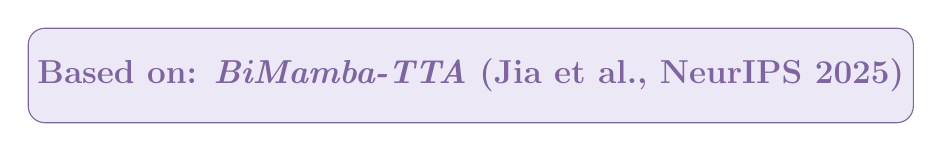
\begin{tikzpicture}
				\node[draw=coolpurple, fill=lightpurple, rounded corners=6pt,
				minimum width=10cm, minimum height=1.2cm,
				font=\large\bfseries, text=coolpurple] {
					Based on: \textit{BiMamba-TTA} (Jia et al., NeurIPS 2025)
				};
			\end{tikzpicture}
		\end{center}
		\vspace{0.3em}
		\begin{columns}
			\begin{column}{0.6\textwidth}
				\textbf{Original setting:} multi-modal physiological signals (EEG, ECG, GSR) for \textit{emotion classification}.
				
				\vspace{0.5em}
				\textbf{Our adaptation:} same family of methods applied to \hl{continuous engagement regression} with richer modalities.
				
				\vspace{0.5em}
				Two key innovations we are adapting:
				\begin{enumerate}
					\item \textbf{BiMamba} - bidirectional selective state-space model for temporal + cross-modal fusion
					\item \textbf{TTA} - test-time adaptation for missing-modality robustness and domain shift
				\end{enumerate}
			\end{column}
			\begin{column}{0.35\textwidth}
				\centering
				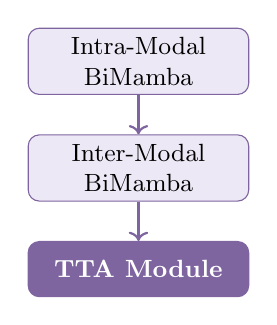
\begin{tikzpicture}[node distance=0.5cm, font=\small]
					\node[draw=coolpurple, fill=lightpurple, rounded corners, minimum width=2.8cm, minimum height=0.7cm, align=center] (intra) {Intra-Modal\\BiMamba};
					\node[draw=coolpurple, fill=lightpurple, rounded corners, minimum width=2.8cm, minimum height=0.7cm, align=center, below=of intra] (inter) {Inter-Modal\\BiMamba};
					\node[draw=coolpurple, fill=coolpurple, rounded corners, minimum width=2.8cm, minimum height=0.7cm, align=center, below=of inter, text=white, font=\small\bfseries] (tta) {TTA Module};
					\draw[->, thick, coolpurple] (intra) -- (inter);
					\draw[->, thick, coolpurple] (inter) -- (tta);
				\end{tikzpicture}
			\end{column}
		\end{columns}
	\end{frame}
	
	\begin{frame}{Foundation: SSMs and Mamba's Selective Attention}
		\begin{columns}[onlytextwidth]
			\begin{column}{0.60\textwidth}
				\textbf{State Space Models (SSMs)} maintain a running \hl{hidden state} - a compressed memory of everything seen so far.
				\vspace{0.3em}
				\begin{itemize}
					\item At each time step: new input + memory $\to$ updated memory + output.
					\item Efficient for \textbf{long sequences} (25 Hz over minutes).
					\item \textit{Unlike RNNs:} the state transition is \textbf{linear} (matrix multiply, no nonlinearity), so SSMs can be computed as a \textbf{convolution during training} - fully parallel - while still running recurrently at inference.
					\item In \textit{"The Hidden Attention of Mamba Models"} by Ali et al. the authors showed that mamba basically self-induces attention.
				\end{itemize}
			\end{column}
			\begin{column}{0.38\textwidth}
				\raggedright
				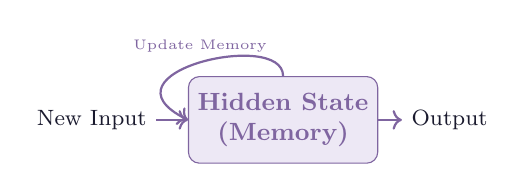
\begin{tikzpicture}[font=\small]
					\node[draw=coolpurple, fill=lightpurple, rounded corners, minimum width=2.2cm, minimum height=1.1cm, align=center, font=\small\bfseries, text=coolpurple] (box) {Hidden State\\(Memory)};
					\node[left=0.4cm of box, text=darktext, font=\footnotesize] (in) {New Input};
					\node[right=0.3cm of box, text=darktext, font=\footnotesize] (out) {Output};
					\draw[->, thick, coolpurple] (in) -- (box);
					\draw[->, thick, coolpurple] (box) -- (out);
					\draw[->, thick, coolpurple] (box.north) .. controls +(0,0.6) and +(-1.2,0.6) .. node[above, font=\tiny, text=coolpurple] {Update Memory} (box.west);
				\end{tikzpicture}
			\end{column}
		\end{columns}
	\end{frame}
	
	\begin{frame}{BiMamba Architecture: Two Levels of Fusion}
		\begin{columns}
			\begin{column}{0.5\textwidth}
				\textbf{Step 1 - Intra-Modal (within each stream)}
				\begin{itemize}
					\item Each modality (e.g. OpenFace2, eGeMaps) is processed \textit{independently}.
					\item \hl{Bidirectional} scan: look forward \textit{and} backward in time to capture context.
				\end{itemize}
				\vspace{0.3em}
				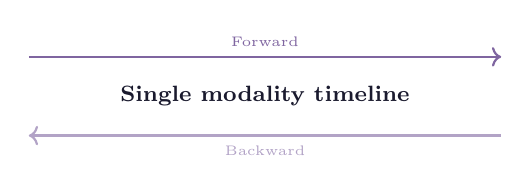
\begin{tikzpicture}
					\node at (0,0) [text=darktext, font=\footnotesize\bfseries] {Single modality timeline};
					\draw[->, thick, coolpurple] (-3,0.5) -- (3,0.5) node[midway, above, font=\tiny] {Forward};
					\draw[<-, thick, coolpurple!60] (-3,-0.5) -- (3,-0.5) node[midway, below, font=\tiny, text=coolpurple!60] {Backward};
				\end{tikzpicture}
			\end{column}
			\begin{column}{0.5\textwidth}
				\textbf{Step 2 - Inter-Modal (across streams)}
				\begin{itemize}
					\item After per-modality encoding, streams are \textit{stacked}.
					\item Mamba sweeps \hl{across} modalities to share cross-modal information.
					\item E.g. audio and face often co-vary during engagement.
				\end{itemize}
				\vspace{0.3em}
				\centering
				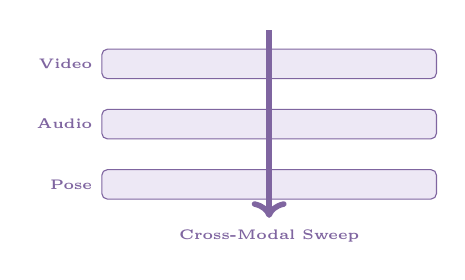
\begin{tikzpicture}[scale=0.85]
					\foreach \y/\lbl in {0.9/Video, 0/Audio, -0.9/Pose} {
						\draw[fill=lightpurple, draw=coolpurple, rounded corners=2pt] (-2.5, \y-0.22) rectangle (2.5, \y+0.22);
						\node[left, text=coolpurple, font=\tiny\bfseries] at (-2.5, \y) {\lbl};
					}
					\draw[->, line width=2pt, coolpurple] (0, 1.4) -- (0, -1.4) node[below, font=\tiny\bfseries, text=coolpurple] {Cross-Modal Sweep};
				\end{tikzpicture}
			\end{column}
		\end{columns}
	\end{frame}
	
	\begin{frame}{Test-Time Adaptation - Why and How}
		\begin{columns}
			\begin{column}{0.45\textwidth}
				\begin{block}{Training (NoXi - Europe)}
					Clean features, known distribution. Model is well-calibrated.
				\end{block}
				\vspace{0.3em}
				\begin{block}{Testing (NoXi+J - Japan/China)}
					New cultural cues, different paralinguistics. \hl{Distribution shift.} Sensors may also go missing.
				\end{block}
			\end{column}
			\begin{column}{0.1\textwidth}
				\centering \Large $\Rightarrow$
			\end{column}
			\begin{column}{0.4\textwidth}
				\textbf{Solution: TTA - adapt on the fly at test time.}
				\vspace{0.5em}
				\begin{enumerate}
					\item \textbf{Smart filter}: keep samples that are \textit{confident} overall but \textit{uncertain} within individual modalities.
					\item \textbf{Mutual-info sharing}: let intact modalities guide corrupted ones.
					\item \textbf{Surgical fine-tuning}: update only BatchNorm + first convolution + first FC of inter-modal block. Core BiMamba weights stay frozen.
				\end{enumerate}
			\end{column}
		\end{columns}
	\end{frame}
	
	\begin{frame}{\textsc{Part 3:} Current Work}
		\begin{center}
			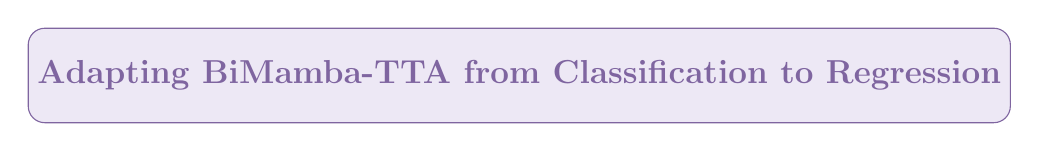
\begin{tikzpicture}
				\node[draw=coolpurple, fill=lightpurple, rounded corners=6pt,
				minimum width=10cm, minimum height=1.2cm,
				font=\large\bfseries, text=coolpurple] {
					Adapting BiMamba-TTA from Classification to \textbf{Regression}
				};
			\end{tikzpicture}
		\end{center}
		\vspace{0.5em}
		The original paper uses \textbf{Shannon entropy} on softmax class probabilities.
		We predict a \textit{continuous} engagement score - so we need a different uncertainty measure.
		
		\vspace{0.5em}
		\begin{block}{Our approach}
			Each prediction head outputs a \textbf{Gaussian predictive distribution}:
			$$p(y \mid x) = \mathcal{N}(\hat{\mu}(x), \hat{\sigma}^2(x))$$
			We use the predicted variance $\hat{\sigma}^2(x)$ as our uncertainty proxy - it is strictly monotone with differential entropy, more numerically stable, and cheaper to compute.
		\end{block}
	\end{frame}
	
	\begin{frame}{Uncertainty Measure: Differential Entropy}
		For a \textit{continuous} distribution we use \textbf{differential entropy}:
		$$H(p) = -\int_{-\infty}^{\infty} p(y) \log p(y) dy$$
		\vspace{0.1em}
		\begin{columns}
			\begin{column}{0.48\textwidth}
				\begin{block}{Interpretation}
					\small
					\begin{itemize}
						\item Measures the \textbf{spread} of a continuous distribution - narrow and peaked $\to$ low entropy; broad and flat $\to$ high entropy.
						\item Unlike discrete entropy, it can be \textbf{negative} and is not invariant under reparametrisation.
						\item Still valid as a \textit{relative} measure of uncertainty within the same distribution family.
					\end{itemize}
				\end{block}
			\end{column}
			\begin{column}{0.48\textwidth}
				\begin{block}{Closed form for a Gaussian}
					\small
					For $\mathcal{N}(\hat{\mu}, \hat{\sigma}^2)$:\\
					
					\vspace{0.75em}
					
					\hspace{0.55em} $H = \frac{1}{2} \ln(2\pi e \hat{\sigma}^2) = \frac{1}{2} \ln(2\pi e) + \frac{1}{2} \ln \hat{\sigma}^2$
					
					\vspace{0.2em}
					
					\begin{itemize}
						\item The mean $\hat{\mu}$ cancels entirely - only \textbf{spread} matters.
						\item $H$ is strictly increasing in $\hat{\sigma}^2$, so we use $\hat{\sigma}^2$ directly as our uncertainty proxy - identical ranking, cheaper to compute.
					\end{itemize}
				\end{block}
			\end{column}
		\end{columns}
	\end{frame}
	
	\begin{frame}{Uncertainty Estimation: Why and How}
		The TTA filter requires knowing how \textit{confident} the model is - both overall and per-modality. Classification had entropy over softmax probabilities; we need a regression analogue.
		\vspace{0.4em}
		
		Three standard approaches, ordered by cost:
		\vspace{0.3em}
		\begin{columns}
			\begin{column}{0.31\textwidth}
				\begin{block}{(a) Dual-Head \\ \small Nix \& Weigend 1994}
					\small Each head outputs $(\hat{\mu}, \ln \hat{\sigma}^2)$. Trained end-to-end with NLL loss:
					$$\mathcal{L}_{NLL} = \frac{1}{2} \ln \hat{\sigma}^2 + \frac{(y - \hat{\mu})^2}{2 \hat{\sigma}^2}$$
					No extra forward passes. Primarily captures \textbf{aleatoric} uncertainty. \hl{Start here.}
				\end{block}
			\end{column}
			\begin{column}{0.31\textwidth}
				\begin{block}{(b) MC Dropout \\ \small Gal \& Ghahramani 2015}
					\small Dropout stays \textit{on} at test time; run $T = 10$-$20$ forward passes. Variance across passes exposes the \hl{epistemic} component. Costs $T \times$ inference time.
					\vspace{0.4em}
					
					Layer on top of (a) if model stalls on NoXi+J.
				\end{block}
			\end{column}
			\begin{column}{0.31\textwidth}
				\begin{block}{(c) Deep Ensembles \\ \small Lakshminarayanan 2016}
					\small Train $K$ independent models; combine predictions. Best calibration in practice, but costs $K \times$ training compute and memory.
					\vspace{0.4em}
					
					Overkill unless (a) and (b) fall short.
				\end{block}
			\end{column}
		\end{columns}
	\end{frame}
	
	\begin{frame}{TTA for Regression: Sample Selection \& Loss}
		\begin{block}{Step 1 - Two-level sample filter (variance replaces entropy)}
			\vspace{0.2em}
			\centering
			$S(x) = \mathbb{I}\{ \hat{\sigma}^2_{multi} \leq \gamma_m \text{ AND } \sum_i w_i \hat{\sigma}^2_i \geq \gamma_u \}$
			\smallskip
			\begin{itemize}
				\item Low multimodal variance $\to$ confident overall (small shift).
				\item High average unimodal variance $\to$ needs cross-modal help.
			\end{itemize}
		\end{block}
		\vspace{0.3em}
		\begin{block}{Step 2 - Regression mutual-info loss via KL between Gaussians}
			\vspace{0.2em}
			\centering
			$\mathcal{L}_{mis} = \sum_i D_{KL}(\mathcal{N}(\hat{\mu}_i, \hat{\sigma}_i^2) \| \frac{1}{2} (\mathcal{N}(\hat{\mu}'_i, \hat{\sigma}'^2_i) + \mathcal{N}(\hat{\mu}_m, \hat{\sigma}^2_m)))$
			\smallskip
			
			\raggedright\small $\hat{\mu}'_i$ = leave-one-out prediction from the other $M-1$ modalities.
		\end{block}
		\vspace{0.3em}
		\begin{block}{Final test-time objective}
			\vspace{0.2em}
			\centering
			$\mathcal{L}_{test}(x) = \alpha(x) \mathbb{I}\{S(x)\} (U_{multi}(x) + \lambda \mathcal{L}_{mis}(x)), \quad \alpha(x) = \frac{1}{\exp(\hat{\sigma}^2_{multi}(x) - Ent_0)}$
		\end{block}
	\end{frame}
	
	\begin{frame}{Why Uncertainty Type Matters for Adaptation}
		\begin{columns}
			\begin{column}{0.48\textwidth}
				\begin{block}{Aleatoric uncertainty}
					Irreducible noise in the data itself. \\
					\textit{Sources:} annotator disagreement, dropped frames, compression. \\
					\vspace{0.3em}
					Adapting on high-aleatoric samples $\to$ \hl{noisy gradients}, wasted capacity.
				\end{block}
			\end{column}
			\begin{column}{0.48\textwidth}
				\begin{block}{Epistemic uncertainty}
					The model hasn't seen this kind of input before. Reducible with more data. \\
					\vspace{0.3em}
					Adapting on high-epistemic samples $\to$ \hl{genuine domain correction}, exactly what we want.
				\end{block}
			\end{column}
		\end{columns}
		\vspace{0.8em}
		\begin{center}
			\textbf{Ideal target sample:} low aleatoric (clean signal) + high epistemic (not observed yet)
		\end{center}
		\vspace{0.3em}
		The dual-head gives us \textit{total} variance; MC Dropout lets us \hl{decompose} it into aleatoric + epistemic so we can filter more precisely for the NoXi $\to$ NoXi+J shift.
	\end{frame}
	
	\begin{frame}{Modality Analysis: Which Streams Are Most Personal?}
		We want to know \textit{which modalities} vary most in predictive power across subjects - to guide where cross-modal fusion and personalisation matter most.
		\vspace{0.4em}
		\begin{columns}
			\begin{column}{0.50\textwidth}
				\textbf{Method:}
				\begin{enumerate}
					\item For each subject $s$ and modality $m$: train a unimodal regressor, compute Pearson correlation $perf_{s,m}$.
					\item Compute per-modality variance across all subjects:
					$$Var_m = \frac{1}{|S|} \sum_s (perf_{s,m} - \overline{perf}_m)^2$$
				\end{enumerate}
				
			\end{column}
			\begin{column}{0.46\textwidth}
				\textbf{Interpretation:}
				\vspace{0.3em}
				\begin{itemize}
					\item \textbf{Small} $Var_m$ $\to$ modality predicts engagement similarly for everyone $\to$ low subject-specificity.
					\vspace{0.4em}
					\item \textbf{Large} $Var_m$ $\to$ modality works well for some subjects and poorly for others $\to$ \hl{highly person-specific}.
					\vspace{0.4em}
					\item High-variance modalities are exactly where cross-modal fusion and personalisation bring the biggest gains.
				\end{itemize}
			\end{column}
		\end{columns}
	\end{frame}
	
	\begin{frame}{Summary}
		\begin{columns}
			\begin{column}{0.32\textwidth}
				\begin{block}{What we're doing}
					\small
					Continuous engagement prediction from multimodal streams in expert-novice interactions, with a focus on cross-cultural personalisation (NoXi $\to$ NoXi+J).
				\end{block}
			\end{column}
			\begin{column}{0.32\textwidth}
				\begin{block}{Architecture}
					\small
					BiMamba: bidirectional Mamba for intra-modal temporal modelling + inter-modal cross-stream fusion, with a TTA module for test-time adaptation.
				\end{block}
			\end{column}
			\begin{column}{0.32\textwidth}
				\begin{block}{Current focus}
					\small
					Adapting TTA to regression via Gaussian heads and differential entropy; analysing per-modality subject-variance to guide personalisation priorities.
				\end{block}
			\end{column}
		\end{columns}
		\vspace{1em}
		\begin{center}
			
\begin{tikzpicture}
				\node[draw=coolpurple, fill=lightpurple, rounded corners=6pt,
				minimum width=6cm, minimum height=1.2cm,
				font=\Large\bfseries, text=coolpurple] {
					Start coding!
				};
			\end{tikzpicture}
		\end{center}
	\end{frame}
	
\end{document}